%% Преамбула TeX-файла

% 1. Стиль и язык
\documentclass[utf8x, times, 14pt]{G7-32} % Стиль (по умолчанию будет 14pt)
\bibliographystyle{gost780u}

% Остальные стандартные настройки убраны в preamble.inc.tex.
\include{preamble.inc}

% Настройки листингов.
\ifPDFTeX
\include{listings.inc}
\else
\usepackage{local-minted}
\fi

% Полезные макросы листингов.
%\include{macros.inc}
%\usepackage{unicode-math}
\DeclareMathOperator*{\Dap}{Δ P_c}

% Стиль титульного листа и заголовки
%\include{00-title}


\begin{document}

\frontmatter % выключает нумерацию ВСЕГО; здесь начинаются ненумерованные главы: реферат, введение, глоссарий, сокращения и прочее.

\maketitle %создает титульную страницу


%\begin{executors}
%\personalSignature{Первый исполнитель}{ФИО}
%
%\personalSignature{Второй исполнитель}{ФИО}
%\end{executors}


%\listoffigures                         % Список рисунков

%\listoftables                          % Список таблиц

%\NormRefs % Нормативные ссылки 
% Команды \breakingbeforechapters и \nonbreakingbeforechapters
% управляют разрывом страницы перед главами.
% По-умолчанию страница разрывается.

% \nobreakingbeforechapters
% \breakingbeforechapters

%\include{00-abstract}

\tableofcontents

%\printnomenclature % Автоматический список сокращений



\include{00-intro}

\mainmatter % это включает нумерацию глав и секций в документе ниже

\chapter{Характеристика исходных данных курсового проекта}
\label{cha:ish_dannie}

\section{Исходные данные для проектирования}

Электрическая сеть сооружается в Костромской области на железобетонных опорах.

\begin{figure}[h]
	\centering
	\includegraphics[width=0.7\textwidth]{inc/svg/scheme}
	\caption{Схема расположения пунктов}
	\label{fig:scheme}
\end{figure}

Питание района электроэнергией будет осуществляться от шин 220 кВ подстанции "К" работающей в составе электроэнергетической системы. Источник питания в режиме наибольших нагрузок обеспечивает полную выдачу необходимой для потребителей активной мощности, а также 87 Мвар реактивной мощности. На шинах источника питания района в режиме наибольших нагрузок обеспечивается напряжение, равно 110 \%, а в режиме наименьших нагрузок 100 \% от номинального.

Для всех пунктов наименьшая нагрузка принимается 37 \% от наибольшей; число часов использования наибольших нагрузок составляет \(4350\; \frac{\textup{ч}}{\textup{год}}\).

Вторичное напряжение на всех сооружаемых подстанциях 10 кВ.

\section{Исходные данные по климатическим условиям и нагрузкам в пунктах потребления}

Электрическая сеть сооружается в Костромской области на железобетонных опорах.

Среднеянварская температура: \(-11,8 ^oC\)

Среднегодовая температура: \(2,7\; ^oC\)

Среднеиюльская температура: \(17,6\; ^oC\)

Район по ветру: I

Район по гололёду: I

%%% Local Variables:
%%% mode: latex
%%% TeX-master: "rpz"
%%% End:
\chapter{Формирование конкурентных вариантов схем сети, включая выбор номинального напряжения участков сети}
\label{cha:var_scheme}

\section{Разработка вариантов схем сети}

В рамках данного курсового проекта необходимо сформировать два варианта схем электрической сети включающих в себя как сети радиально-магистрального типа, так и кольцевую сеть.

Поскольку в составе потребителей всех пунктов имеется нагрузка I и II категории надежности, для обеспечения бесперебойности электроснабжения согласно пункту п. 1.2.19 и п. 1.2.20 ПУЭ \cite{пуэ7} требуется предусмотреть возможность получения электроэнергии от двух независимых взаимнорезервирующих источников питания. Это требование исключает возможность применения одноцепных линий в составе разомкнутых сетей радиально-магистрального типа. Таким образом, проектируемая районная электрическая сеть должна содержать участки двухцепных радиально-магистральных линий, либо сформированные в кольцевую сеть одноцепные линии.

Выбор среди конкурирующих вариантов осуществляется, опираясь на технические и технико-экономические показатели:
\begin{itemize}
	\item передача электроэнергии потребителям должна осуществляться по возможно кратчайшему пути, что обеспечивает снижение стоимости сооружения линий и экономию потерь мощности и электроэнергии;
	\item схема сети должна обеспечивать требуемый уровень надежности электроснабжения потребителей;
	\item схема сети должна быть по возможности (обснованно) простой;
	\item следует стремиться к минимизации количества трансформаций напряжения, что снижает необходимую установленную мощность трансформаторов и автотрансформаторов и, соответственно, капиталовложения на сооружение сети, а также - потери мощности и электроэнергии;
	\item не допускается сооружение линий по параллельным, рядом идущим трассам;
	\item следует избегать строительства малозагруженных линий, используемых только во время отключения элементов сети;
	\item не рекомендуется сооружать кольцевые сети, обеспечивающие электроснабжение 4-5 подстанций, из-за недопустимо больших потерь напряжения в послеаварийных режимах;
	\item комплекс номинального напряжения и схемы сети должны обеспечивать необходимое качество электроснабжения потребителей и выполнение технических ограничений по параметрам электрооборудования линий и подстанций;
	\item возможность сохранения принятых решений по развитию сети при небольших отклонениях нагрузок от прогнозируемых.
\end{itemize}

Изобразим возможные варианты схем районных сетей для наших исходных данных на рисунке \ref{fig:variant_scheme}.

Первый вариант [рисунок \ref{fig:variant_scheme} (а)] "--- кольцевая схема сети. Данный вариант соответствует требованиям по уровню надежности, обладает малым количеством числа трансформации уровней напряжения. Так же этот вариант обладает простыми схемами транзитных распределительных устройств (РУ). К недостатком такой схемы сети можно отнести повышенные потери мощности и электроэнергии и большими потерями напряжения в послеаварийных режимах, а также повышенная длина трасс линий.

Второй вариант [рисунок \ref{fig:variant_scheme} (б)] "--- радиально-магистральная схема сети с небольшой кольцевой сетью в конце. Такой вариант мы сразу можем отбросить, так как не допускается сооружение линий по рядом идущим трассам.

Третий вариант [рисунок \ref{fig:variant_scheme} (в)] "--- схема сети радиально-магистрального типа. Такие схемы обладают наименьшей длиной трасс линий, наименьшими потерями напряжения, мощности и электроэнергии и большими резервами по пропускной способности линий при перспективном росте нагрузок в заданных пунктах по сравнению с кольцевыми сетями. Однако этот вариант не рекомендуется к выбору, так как в нем соединяются все 5 ПС в одну линию, что из опыта проектирования ведет к тому, что на дальних пунктах тяжело поддерживается нужное напряжение.

Четвертый вариант [рисунок \ref{fig:variant_scheme} (г)] "--- является более оптимальной радиально-магистральной схемой сети, по сравнению с предыдущим вариантом, так как она лишена недостатка поддержания напряжения на последней ПС.

Таким образом, можем сделать вывод, что наиболее целесообразными конкурентными схемами, будут первая и четвертая (рисунки \ref{fig:variant_scheme} (а) и (г) соответственно), далее схемы №1 и №2.

\begin{figure}[h]
	\centering
	\includegraphics[width=0.7\textwidth]{inc/svg/variant_scheme}
	\caption{Варианты схем районных сетей}
	\label{fig:variant_scheme}
\end{figure}


\section{Выбор номинальных напряжений участков сети}

Экономически целесообразное номинальное напряжение участка сети зависит от некоторых параметров, среди которых основными являются передаваемая активная мощность по одной цепи линии и длина линии электропередачи.

\begin{table}[ht]
	\small
	\caption{Ориентировочные значения длин линий, дальности электропередачи и передаваемых мощностей для номинальных напряжений 35-220 кВ электрических сетей}
	\begin{tabularx}{\textwidth}{|X|Z|Z|Z|}
		\hline
		Номинальное напряжение, кВ & Экономически целесообразная передаваемая мощность на одну цепь линии, МВт & Средняя длина линий между соседними подстанциями, км & Средняя дальность электропередачи, км \\ \hline
		35 & 3 "--- 8 & 10 & 20 \\ \hline
		110 & 10 "--- 45 & 25 & 75 \\ \hline
		220 & 70 "--- 140 & 100 & 200 \\ \hline
	\end{tabularx}
	\label{tab:orient_l}
\end{table}

\subsection{Расчет для схемы №1:}

Выполним предварительный расчет потокораспределения активной мощности, передаваемой по одной цепи каждой линии, при котором допускается не учитывать потери мощности в сети.
\[P_{4-5}^{\textup{1ц}} = \frac{P_5}{2} = \frac{35}{2} = 17,5\; \textup{МВт}\]
\[P_{3-4}^{\textup{1ц}} = \frac{P_4 + P_5}{2} = \frac{40 + 35}{2} = 37,5\; \textup{МВт}\]
	
Для предварительного расчета потокораспределения активной мощности в кольцевой сети К-1-3-2-К представим нагрузки пунктов 3-4-5 в виде нагрузки одного эквивалентного пункта 3':
\[P_3{'} = P_3 + P_4 + P_5 = 30 + 40 + 35 = 105\; \textup{МВт}\]

Вычислим активную мощность передаваемую по головным участкам кольцевой сети. Принимаем во внимание, что на этапе проектирования, когда сечение проводов ЛЭП еще не выбраны, для всех линий кольцевой сети, разрешается рассчитывать предварительное потокораспределение по длинам линии вместо сопротивлений.

Для участка K-1:
%\begin{eqndesc}[H]
\begin{equation*}
	\begin{split}
		P_\textup{К-1} &= \frac{P_1(L_{13} + L_{23} + L_\textup{К'-2}) + P_3{'}(L_{23} + L_\textup{К'-2}) + P_2\cdot L_\textup{К'-2}}{L_\textup{К-1} + L_{13} + L_{23} + L_\textup{К'-2}} = \\
			  &= \frac{70(49,2 + 41,8 + 49,2) + 105(41,8 + 49,2) + 70\cdot 49,2}{41,8 + 49,2 + 41,8 + 49,2} = 125,3\; \textup{МВт}
	\end{split}
\end{equation*}
%\end{eqndesc}

Для участка К'-2:
\begin{equation*}
	\begin{split}
		P_\textup{К'-2} &= \frac{P_2(L_{23} + L_{13} + L_\textup{К-1}) + P_3{'}(L_{13} + L_\textup{К-1}) + P_1\cdot L_\textup{K-1}}{L_\textup{К-1} + L_{13} + L_{23} + L_\textup{К'-2}} = \\
		&= \frac{70(41,8 + 49,2 + 41,8) + 105(49,2 + 41,8) + 70\cdot 41,8}{41,8 + 49,2 + 41,8 + 49,2} = 119,7\; \textup{МВт}
	\end{split}
\end{equation*}

Проверим правильность полученных результатов расчета активной мощности на головных участках кольцевой сети посредством оценки баланса мощности:
\[P_\textup{К-1} + P_\textup{К'-2} = 125,3 + 119,7 = 245\; \textup{МВт}\]
\[P_1 + P_3{'} + P_2 = 70 + 105 + 70 = 245\; \textup{МВт}\]
проверка сошлась

Теперь определим потокораспределение активной мощности на участках 1-3 и 2-3:
\[P_{13} = P_\textup{K-1} - P_1 = 125,3 - 70 = 55,3\; \textup{МВт}\]
\[P_{23} = P_\textup{K'-1} - P_2 = 119,7 - 70 = 49,7\; \textup{МВт}\]

Так как \(P_{13} > 0\) и \(P_{23} > 0\), то точка потокораздела находтся в третьем пункте потребления.

Полученные результаты предварительного потокораспределения активной мощности для удобства последующих рассуждений о выборе номинального напряжения сведем в табл. \ref{tab:vybor_u_n1}

\begin{table}[H]
	\small
	\caption{Выбор номинального напряжения участков сети}
	\begin{tabularx}{\textwidth}{|l|Z|Z|Z|Z|Z|Z|}
		\hline
		Линия                  & K1    & K2    & 13   & 23   & 34   & 45   \\ \hline
		\(P_\textup{1ц}\) МВт  & 125,3 & 119,7 & 55,3 & 49,7 & 37,5 & 17,5 \\ \hline
		L, км                  & 41,8  & 49,2  & 49,2 & 41,8 & 25,9 & 25,9 \\ \hline
		\(U_\textup{ном}\), кВ & 220   & 220   & 110  & 110  & 110  & 110  \\ \hline
	\end{tabularx}
	\label{tab:vybor_u_n1}
\end{table}

Все участки кольцевой сети следует проектировать на одно номинальное напряжение, выбираемое по наиболее загруженным головным участкам. Поскольку по головным участкам кольцевой сети К-1, К-2 длиной 41,8 и 49,2 км передается активная мощность более 70 МВт, в соответствии с таблицей \ref{tab:orient_l} для всех участков кольцевой сети следует выбрать номинальное напряжение 220 кВ.

\subsection{Расчет для схемы №2:}

Участок 4-5:
\[P_{4-5}^\textup{1ц} = \frac{P_5}{2} = \frac{70}{2} = 35\; \textup{МВт}\]

Участок 3-4:
\[P_{3-4}^\textup{1ц} = \frac{P_4 + P_5}{2} = \frac{40 + 35}{2} = 37,5\; \textup{МВт}\]

Участок 3-2:
\[P_{3-2}^\textup{1ц} = \frac{P_2}{2} = \frac{70}{2} = 35\; \textup{МВт}\]

Участок 1-3:
\[P_{1-3}^\textup{1ц} = \frac{P_2 + P_3 + P_4 + P_5}{2} = \frac{70 + 30 + 40 + 35}{2} = 87,5\; \textup{МВт}\]

Участок К-1:
\[P_\textup{K-2}^\textup{1ц} = \frac{P_1 + P_2 + P_3 + P_4 + P_5}{2} = \frac{70 + 70 + 30 + 40 + 35}{2} = 122,5\; \textup{МВт}\]

Аналогично рассчитываем передаваемую мощность в линиях схемы №1 и сводим в таблицу \ref{tab:vybor_u_n2}.

\begin{table}[H]
	\small
	\caption{Выбор номинального напряжения участков сети}
	\begin{tabularx}{\textwidth}{|l|Z|Z|Z|Z|Z|}
		\hline
		Линия                  & K1    & 13   & 32   & 34   & 45   \\ \hline
		\(P_\textup{1ц}\) МВт  & 122,5 & 87,5 & 35   & 37,5 & 35   \\ \hline
		L, км                  & 41,8  & 49,2 & 41,8 & 25,9 & 25,9 \\ \hline
		\(U_\textup{ном}\), кВ & 220   & 220  & 110  & 110  & 110  \\ \hline
	\end{tabularx}
	\label{tab:vybor_u_n2}
\end{table}

%%% Local Variables:&
%%% mode: latex
%%% TeX-master: t
%%% End:
\chapter{Оценка баланса реактивной мощности в проектируемой сети}
\label{cha:ocenka_brm}

На основе оптимизационных расчетов распределения реактивной мощности в электроэнергетической системе для каждого ее узла определяется реактивная мощность, которую целесообразно передавать из электроэнергетической системы в распределительные сети, питающиеся от того или иного узла. Поэтому при проектировании электрической сети, получающей питание от подстанций электроэнергетической системы, задается реактивная мощность \(Q_{\textup{расп}\Sigma}\), которую целесообразно потреблять из системы (в заданном узле присоединения) в режиме наибольших нагрузок, или же коэффициент реактивной мощности. Потребление большей реактивной мощности приведет к дополнительным затратам на передачу этой мощности и, следовательно, к отступлению от оптимального режима питающей системы. В связи с этим, в проекте оценивается выполнение баланса реактивной мощности в проектируемой сети и при необходимости устанавливаются компенсирующие устройства.

\section{Проверка по условию выполнения баланса реактивной мощности в сети}

Потребление реактивной мощности в проектируемой сети в период наибольших нагрузок складывается из заданных реактивных нагрузок в пунктах потребления, рассчитанных с учетом предварительного этапа установки БСК с целью выполнения условия \(\tg\,{\varphi_i} \le \tg\,{\varphi_\textup{пред}}\) и потерь реактивной мощности в линиях и понижающих трансформаторах с учетом зарядных мощностей линий. При определении одновременно потребляемой реактивной мощности следует учитывать несовпадение по времени суток наибольших нагрузок отдельных потребителей.

При четырех и более пунктах потребления среднестатистическое значение коэффициента одновременности реактивных нагрузок на шинах 220 кВ источника питания составляет 0,98 \cite{глазунов_шведов}. Наибольшая суммарная реактивная мощность потребляемая в проектируемой сети в период наибольших нагрузок рассчитывается по формуле:
\begin{eqndesc}[H]
	\begin{equation}
		Q_{\textup{треб}\Sigma} = k_{\textup{одн}Q} \cdot \sum_{i=1}^{n} Q_{\textup{нб}i} + \Delta Q_{\textup{т}\Sigma} + \sum_{j=1}^{m}\left(\Delta Q_{\textup{л}j} - Q_{cj}\right)
		\label{eqn:sum_q_treb}
	\end{equation}

где \(Q_{\textup{нб}i}\) "--- наибольшая реактивная нагрузка \textit{i}-го пункта с учетом установленных конденсаторных батарей по условию не превышения предельных значений коэффициента реактивной мощности;
n "--- число пунктов потребления электроэнергии;
\(k_{\textup{одн}Q}\) "--- коэффициент одновременности наибольших реактивных нагрузок подстанций;
\(\Delta Q_{\textup{т}\Sigma}\) "--- суммарные потери в трансформаторах подстанций сети;
\(Q_{\textup{л}j}\) "--- потери реактивной мощности в \textit{j}-й линии электропередачи;
\(Q_{cj}\) "--- зарядная мощность \textit{j}-й линии электропередачи;
m "--- число линий электропередачи в сети.
\end{eqndesc}

\subsection{Оценка баланса реактивной мощности для варианта схемы сети 1}

а) \textit{Суммарная реактивная нагрузка на шинах 220 кВ источника питания К}:
\[k_{\textup{одн}Q} \cdot  \sum_{i=1}^{5} Q_{\textup{нб}i}^{'} = 0,98 \cdot 95,4 = 93,5\; \textup{МВар}\]

б) Суммарные потери реактивной мощности в трансформаторах проектируемой сети:
\begin{eqndesc}[H]
\[\Delta Q_{\textup{т}\Sigma} = \sum_{i=1}^{n} \Delta Q_{\textup{т}i} \cong 0,08 \sum_{i=1}^{n} m_{\textup{т}i} \cdot S_{\textup{нб}i},\]

где \(m_{\textup{т}i}\) "--- число трансформации \textit{i}-й ПС.
\end{eqndesc}
\[\Delta Q_{\textup{т}\Sigma} = 0,08(1\cdot 75,2 + 1\cdot 75,2 + 1\cdot 32,1 + 2\cdot 43,0 + 2\cdot 37,5) = 27,5\; \textup{МВар}\]

в) Генерация и потери реактивной мощности в ВЛ:

Зарядная мощность в линии рассчитывается по формуле:
\begin{eqndesc}[H]
\begin{equation}
	Q_c = n_\textup{ц} \cdot q_{c0} \cdot L,
	\label{eqn:зарядная_мощность}
\end{equation}

где \(n_\textup{ц}\) "--- количество цепей в линии; \\
\(q_{c0}\) "--- удельная генерация, \(\frac{\textup{МВар}}{\textup{км}}\); \\
\(q_\textup{с0}^{220} = 0,14\; \frac{\textup{МВар}}{\textup{км}}\) - для ВЛ 220 кВ, \(q_{c0}^{110} = 0,036\; \frac{\textup{МВар}}{\textup{км}}\) - для ВЛ 110 кВ.
\end{eqndesc}

Рассчитаем по формуле \eqref{eqn:зарядная_мощность} зарядную мощность в линии К-1:
\[Q_{cK1} = 1 \cdot 0,14 \cdot 41,8 = 5,85\; \textup{МВар}\]

Для оценки потерь реактивной мощности в ВЛ, воспользуемся известным соотношением \cite{глазунов_шведов}:
\begin{eqndesc}[H]
	\begin{equation}
		\frac{\Delta Q_\textup{л}}{Q_c} \cong \left(\frac{P_\textup{л}}{P_\textup{нат}\cdot n_\textup{ц}}\right)^2 \rightarrow \Delta Q_\textup{л} \cong \left(\frac{P_\textup{1ц}}{P_\textup{нат}}\right)^2 \Delta Q_c,
		\label{eqn:потери_реактивной_мощности_вл}
	\end{equation}

где \(P_\textup{нат}\) "--- мощность при передачи которой по одной цепи линии, потери реактивной мощности в сопротивлении линии равны зарядной мощности в линии. \\
\end{eqndesc}

Натуральная мощность для разных уровней напряжения:
\[P_\textup{нат}^{220} = 130\; \textup{МВт}\]
\[P_\textup{нат}^{110} = 30\; \textup{МВт}\]

Для ВЛ 110 кВ с \(P_\textup{1ц} \leq P_\textup{нат}^{110} = 30\; \textup{кВ} \rightarrow \Delta Q_\textup{л} \approx Q_c\). В нашем случае мы можем отбросить линию 4-5, так как \(P_{1c(45)} = 17,5\; \textup{МВт}\leq P_\textup{нат}^{110} = 30\; \textup{МВт}\).

Потери реактивной мощности в линии по формуле \eqref{eqn:потери_реактивной_мощности_вл}:
\[\Delta Q_\textup{лК1} = \left(\frac{P_\textup{1ц(К1)}}{P_\textup{нат}^{220}}\right)^2 \cdot Q_{cK1} = \left(\frac{125,3}{130}\right)^2 \cdot 5,85 = 5,43\; \textup{МВар}\]

Расчет для остальных линий проводится аналогично. Сведем результаты в таблицу \ref{tab:рез_расчета_q_c0}.

\begin{table}[H]
	\small
	\caption{Результаты расчета \(q_\textup{c0}\) и \(\Delta Q_\textup{л}\)}
	\begin{tabularx}{\textwidth}{|l|Z|Z|Z|Z|Z|Z|}
		\hline
		Линия                  & К-1   & К-2   & 1-3  & 2-3  & 3-4  & \(\Sigma\) \\ \hline
		L, км                  & 41,8  & 49,2  & 49,2 & 41,8 & 25,9 & 207,9          \\ \hline
		\(n_\textup{ц}\)       & 1     & 1     & 1    & 1    & 2    & -          \\ \hline
		\(P_\textup{1ц}\), МВт & 125,3 & 119,7 & 55,3 & 49,7 & 37,5 & -        \\ \hline
		\(Q_c\), МВар          & 5,85  & 6,89  & 6,89 & 5,85 & 1,86 & 27,3       \\ \hline
		\(\Delta Q_\textup{л}\), МВар & 5,43 & 5,84 & 1,25 & 0,86 & 2,91 & 16,3 \\ \hline
	\end{tabularx}
	\label{tab:рез_расчета_q_c0}
\end{table}

Суммарное значение разности потерь реактивной мощности в сопротивлениях линий и зарядной мощности линии (без учета ВЛ 4-5):
\[\sum_{j=1}^{5} = (\Delta Q_{\textup{л}j} - Q_{cj}) = 16,3 - 27,3 = -11,0\; \textup{МВар}\]

По формуле \eqref{eqn:sum_q_treb}:
\[Q_{\textup{треб}\Sigma} = 93,5 + 27,5 - 11,0 = 110\; \textup{МВар}\]

Так как \(Q_{\textup{треб}\Sigma} = 110\; \textup{МВар} > Q_{\textup{расп}\Sigma} = 87\; \textup{МВар}\), то в сети требуется установка дополнительных БСК по условию баланса реактивной мощности.

Суммарная мощность требуемых БСК:
\[Q_{\textup{КУдоп}\Sigma} = Q_{\textup{треб}\Sigma} - Q_{\textup{расп}\Sigma} = 110 - 87 = 23,0\; \textup{МВар}\]

г) Расстановка дополнительных компенсирующих устройств (КУ)
Необходимое число дополнительных компенсирующих устройств:
\[N_\textup{БСК}^{\textup{треб}} = \frac{Q_{\textup{КУ}\Sigma}}{1,2} = \frac{23,0}{1,2} = 19,2 \rightarrow N_\textup{БСК} = 20\]

Из условия равенства коэффициентов реактивной мощности нагрузок на шинах 10 кВ \cite{глазунов_шведов}:
\begin{equation}
	\tg\, \varphi_\textup{б} = \frac{\sum_{i=1}^{n} Q_{\textup{нб}i} - Q_{\textup{КУ}\Sigma}}{\sum_{i=1}^{n} P_{\textup{нб}i}} = 0,296
\end{equation}

Тогда мощность устанавливаемых конденсаторных батарей (сверх установленных по условию не превышения предельных значений коэффициента реактивной мощности) на i-й подстанции:
\[Q_{\textup{БСК}i}^{\textup{треб}} = P_{\textup{нб}i}\cdot (\tg\, \varphi_i - \tg \, \varphi_\textup{б})\]

На примере пункта 1 произведем расчет необходимого количества БСК для дополнительной установки:
\[Q_{\textup{БСК1}}^{\textup{треб}} = 70 \cdot (0,391 - 0,296) = 6,65\; \textup{МВар}\]
\[N_\textup{БСК1}^{треб} = \frac{Q_\textup{БСК1}}{1,2} = \frac{6,65}{1,2} = 5,54 \rightarrow N_\textup{БСК1} = 4\]

\begin{table}[H]
	\small
	\caption{Оценка баланса реактивной мощности с учетом установки дополнительных батарей статических конденсаторов}
	\label{tab:нагрузки_с_батареями_кольцо}
	\begin{tabularx}{\textwidth}{|l|Z|Z|Z|Z|Z|Z|}
		\hline
		№ Пункта                               & 1     & 2     & 3     & 4     & 5     & \(\Sigma\) \\ \hline
		\(P_\textup{нб}\), МВт                 & 70    & 70    & 30    & 40    & 35    & 245        \\ \hline
		\(Q_\textup{нб}^{'}\), МВар            & 27,4  & 27,4  & 11,3  & 15,7  & 13,6  & 95,4       \\ \hline
		\(\tg\, \varphi^{'}\)                  & 0,391 & 0,391 & 0,377 & 0,393 & 0,389 & -          \\ \hline
		\multicolumn{7}{|l|}{\(\tg\, \varphi_\textup{б} = 0,296\)}                                  \\ \hline
		\(Q_\textup{ку.доп}\), МВар            & 6,65  & 6,65  & 2,50  & 3,90  & 3,30  & 22,3       \\ \hline
		\(N_\textup{БСК.доп}^{\textup{треб}}\) & 5,54  & 5,54  & 2,08  & 3,25  & 2,75  & 19,2       \\ \hline
		\(N_\textup{БСК.доп}\)                 & 6     & 6     & 2     & 4     & 2     & 20         \\ \hline
		\(Q_\textup{БСК.доп}\), МВар           & 7,2   & 7,2   & 2,4   & 4,8   & 2,4   & 24         \\ \hline
		\(Q_\textup{нб}^{''}\), МВар           & 20,2  & 20,2  & 8,9   & 10,9  & 11,2  & 71,4       \\ \hline
		\(S_\textup{нб}^{''}\), МВА            & 72,9  & 72,9  & 31,3  & 41,5  & 36,7  & -          \\ \hline
		\(Q_\textup{прив}\), МВар              & 26,0  & 26,0  & 46,1  & 14,2  & 14,1  & -          \\ \hline
		\(S_\textup{прив}\), МВар              & 74,7  & 74,7  & 105,2 & 42,4  & 37,7  & -          \\ \hline
	\end{tabularx}
\end{table}

После расстановки на подстанциях проектируемой сети батарей статических конденсаторов по условию выполнения баланса реактивной мощности необходимо определить действительные реактивные и полные нагрузи подстанций \(Q_{\textup{нб}i}^{''}\) и \(S_{\textup{нб}i}^{''}\).

В качестве примера рассчитаем приведенную нагрузку подстанции 1:
\[Q_\textup{бск.доп1} = N_\textup{бск.доп1} \cdot Q_\textup{бк(1)} = 4 \cdot 1,2 = 4,8\; \textup{МВар}\]
\[Q_\textup{нб}^{''} = Q_\textup{нб}^{'} - Q_\textup{бск.доп1} = 27,4 - 4,8 = 22,6\; \textup{МВар}\]
\[S_\textup{нб}^{''} = \sqrt{P_\textup{нб1}^2 + Q_\textup{нб1}^{'2}} = \sqrt{70^2 + 27,4^2} = 73,6\; \textup{МВА}\]
\[Q_\textup{прив1} = Q_\textup{нб1}^{''} + 0,08 \cdot S_\textup{нб1}^{''} = 22,6 + 73,6 \cdot 0,08 = 28,5\; \textup{МВар}\]
\[S_\textup{прив1} = \sqrt{P_\textup{нб1}^2 + Q_\textup{прив1}^2} = \sqrt{70^2 + 28,5^2} = 75,6\; \textup{МВар}\]

Для остальных подстанций 2, 4 и 5 с двухобмоточными трансформаторами расчет выполняется аналогично. Исключение составляет автотрансформаторная подстанция 3, для которой приведенная нагрузка складывается из нагрузок на шинах низшего и среднего напряжения:
\begin{equation*}
	\begin{split}
		Q_\textup{прив3} &= Q_\textup{нб3}^{''} + Q_\textup{прив4} + Q_\textup{прив5} + \\
		&+ 0,08 \sqrt{(P_\textup{нб3} + P_\textup{нб4} + P_\textup{прив5})^2 + (Q_\textup{нб3}^{''} + Q_\textup{прив4} + Q_\textup{прив5})^2} \\
		&= 8,9 + 14,2 + 11,7 + \\
		&+ 0,08 \sqrt{(30 + 40 + 35)^2 + (8,9 + 14,2 + 11,7)^2} = 43,6\; \textup{МВар}
	\end{split}
\end{equation*}

\begin{equation*}
	\begin{split}
		S_\textup{прив3} &= \sqrt{(P_\textup{нб3} + P_\textup{нб4} + P_\textup{нб5})^2 + (Q_\textup{прив3})^2} = \\
		&= \sqrt{(30 + 40 + 35)^2 + (43,6)^2} = 105,2\; \textup{МВА}
	\end{split}
\end{equation*}

\subsection*{Расчет для варианта схемы №2:}

Расчёт для варианта схемы 2 во многом выполняется аналогично варианту схемы 1, поэтому упустим пояснения в некоторых подпунктах

а) Суммарная реактивная нагрузка на шинах 220 кВ источника питания К:
\[k_{\textup{одн}Q} \cdot  \sum_{i=1}^{5} Q_{\textup{нб}i}^{'} = 0,98 \cdot 95,4 = 93,5\; \textup{МВар}\]

б) Суммарные потери реактивной мощности в трансформаторах проектируемой сети:

\[\Delta Q_{\textup{т}\Sigma} = 0,08(1\cdot 75,2 + 2\cdot 75,2 + 1\cdot 32,1 + 2\cdot 43,0 + 2\cdot 37,5) = 33,5\; \textup{МВар}\]

в) Генерация и потери реактивной мощности в ВЛ.

Рассчитаем по формуле \eqref{eqn:зарядная_мощность} зарядную мощность в линии К-1:
\[Q_{cK1} = 2 \cdot 0,14 \cdot 41,8 = 11,7\; \textup{МВар}\]

Потери реактивной мощности в линии по формуле \eqref{eqn:потери_реактивной_мощности_вл}:
\[\Delta Q_\textup{лК1} = \left(\frac{P_\textup{1ц(К1)}}{P_\textup{нат}^{220}}\right)^2 \cdot Q_{cK1} = \left(\frac{122,5}{130}\right)^2 \cdot 11,7 = 10,4\; \textup{МВар}\]

Расчет для остальных линий проводится аналогично. Сведем результаты в таблицу \ref{tab:рез_расчета_q_c0_схема2}.

\begin{table}[H]
	\small
	\caption{Результаты расчета \(q_\textup{c0}\) и \(\Delta Q_\textup{л}\)}
	\begin{tabularx}{\textwidth}{|l|Z|Z|Z|Z|Z|Z|}
		\hline
		Линия                         & К-1   & 1-3  & 3-2  & 3-4  & 4-5  & \(\Sigma\) \\ \hline
		L, км                         & 41,8  & 49,2 & 41,8 & 25,9 & 25,9 & 184,6      \\ \hline
		\(n_\textup{ц}\)              & 2     & 2    & 2    & 2    & 2    & -          \\ \hline
		\(P_\textup{1ц}\), МВт        & 122,5 & 87,5 & 35   & 37,5 & 17,5 & 300        \\ \hline
		\(Q_c\), МВар                 & 11,7  & 13,8 & 3,01 & 1,86 & -    & 32,2       \\ \hline
		\(\Delta Q_\textup{л}\), МВар & 10,9  & 11,7 & 10,2 & 5,10 & -    & 25,5       \\ \hline
	\end{tabularx}
	\label{tab:рез_расчета_q_c0_схема2}
\end{table}

Суммарное значение разности потерь реактивной мощности в сопротивлениях линий и зарядной мощности линии:
\[\sum_{j=1}^{4} = (\Delta Q_{\textup{л}j} - Q_{cj}) = 25,2 - 32,2 = -6,70\; \textup{МВар}\]

По формуле \eqref{eqn:sum_q_treb}:
\[Q_{\textup{треб}\Sigma} = 93,5 + 33,5 - 6,70 = 120,3\; \textup{МВар}\]

Так как \(Q_{\textup{треб}\Sigma} = 120,3\; \textup{МВар} > Q_{\textup{расп}\Sigma} = 87\; \textup{МВар}\), то в сети требуется установка дополнительных БСК по условию баланса реактивной мощности.

Суммарная мощность требуемых БСК:
\[Q_{\textup{КУдоп}\Sigma} = Q_{\textup{треб}\Sigma} - Q_{\textup{расп}\Sigma} = 120,3 - 87 = 33,3\; \textup{МВар}\]

г) Расстановка дополнительных КУ

Из условия равенства коэффициентов реактивной мощности нагрузок на шинах 10 кВ \cite{глазунов_шведов}:
\begin{equation}
	\tg\, \varphi_\textup{б} = \frac{\sum_{i=1}^{n} Q_{\textup{нб}i} - Q_{\textup{КУ}\Sigma}}{\sum_{i=1}^{n} P_{\textup{нб}i}} = 0,253
\end{equation}

Необходимое число дополнительных КУ:
\[N_\textup{БСК}^{\textup{треб}} = \frac{Q_{\textup{КУ}\Sigma}}{1,2} = \frac{33,3}{1,2} = 27,8 \rightarrow N_\textup{БСК} = 42\]

Мощность устанавливаемых БСК (сверх установленных по условию не превышения предельных значений коэффициента реактивной мощности) на i-й подстанции:
\[Q_{\textup{БСК}i}^{\textup{треб}} = P_{\textup{нб}i}\cdot (\tg\, \varphi_i - \tg \, \varphi_\textup{б})\]

На примере пункта 1 произведем расчет необходимого количества БСК для дополнительной установки:
\[Q_{\textup{БСК1}}^{\textup{треб}} = 70 \cdot (0,391 - 0,253) = 9,7\; \textup{МВар}\]
\[N_\textup{БСК1}^{треб} = \frac{Q_\textup{БСК1}}{1,2} = \frac{9,7}{1,2} = 8,1 \rightarrow N_\textup{БСК1} = 8\]
\[Q_\textup{БСК1} = N_\textup{БСК1} \cdot 1,2 = 8 \cdot 1,2 = 9,6\; \textup{МВар}\]
\[Q_\textup{нб1}^{''} = Q_\textup{нб1}^{'} - Q_\textup{БСК1} = 27,4 - 9,6 = 17,8\; \textup{МВар}\]


\begin{table}[H]
	\small
	\caption{Оценка баланса реактивной мощности с учетом установки дополнительных батарей статических конденсаторов.}
	\begin{tabularx}{\textwidth}{|l|Z|Z|Z|Z|Z|Z|}
		\hline
		№ Пункта                           & 1     & 2     & 3     & 4     & 5     & \(\Sigma\) \\ \hline
		\(P_\textup{нб}\), МВт             & 70    & 70    & 30    & 40    & 35    & 245        \\ \hline
		\(Q_\textup{нб}^{'}\), МВар        & 27,4  & 27,4  & 11,3  & 15,7  & 13,6  & 95,4       \\ \hline
		\(\tg\, \varphi^{'}\)              & 0,391 & 0,391 & 0,377 & 0,393 & 0,389 & -          \\ \hline
		\multicolumn{7}{|l|}{\(\tg\, \varphi_\textup{б} = 0,253\)}                              \\ \hline
		\(Q_\textup{ку.доп}\), МВар        & 9,7   & 9,7   & 3,5   & 5,6   & 4,8   & 33,3       \\ \hline
		\(N_\textup{БСК}^{\textup{треб}}\) & 8,1   & 8,1   & 2,9   & 4,7   & 4,0   & 27,8       \\ \hline
		\(N_\textup{БСК}\)                 & 8     & 8     & 2     & 6     & 4     & 28         \\ \hline
		\(Q_\textup{БСК.доп}\), МВар       & 9,6   & 9,6   & 2,4   & 7,2   & 4,8   & 33,6       \\ \hline
		\(Q_\textup{нб}^{''}\), МВар       & 17,8  & 17,8  & 8,9   & 8,5   & 8,8   & 61,8       \\ \hline
		\(S_\textup{нб}^{''}\), МВА        & 72,2  & 72,2  & 31,3  & 40,9  & 36,1  & -          \\ \hline
		\(Q_\textup{прив}\), МВар          & 23,6  & 23,6  & 70,7  & 11,8  & 11,7  & -          \\ \hline
		\(S_\textup{прив}\), МВар          & 73,9  & 73,9  & 175,2 & 41,7  & 36,9  & -          \\ \hline
	\end{tabularx}
\end{table}

После расстановки на подстанциях проектируемой сети батарей статических конденсаторов по условию выполнения баланса реактивной мощности необходимо определить действительные реактивные и полные нагрузи подстанций \(Q_{\textup{нб}i}^{''}\) и \(S_{\textup{нб}i}^{''}\).

В качестве примера рассчитаем приведенную нагрузку подстанции 1:
\[Q_\textup{БСК1} = N_\textup{БСК1} \cdot 1,2 = 10 \cdot 1,2 = 12\; \textup{МВар}\]
\[Q_\textup{нб1}^{''} = Q_\textup{нб1}^{'} - Q_\textup{БСК1} = 27,4 - 12 = 15,4\; \textup{МВар}\]
\[S_\textup{нб}^{''} = \sqrt{P_\textup{нб1}^2 + Q_\textup{нб1}^{''}} = \sqrt{70^2 + 15,4^2} = 71,7\; \textup{МВА}\]
\[Q_\textup{прив1} = Q_\textup{нб1}^{''} + 0,08 \cdot S_\textup{нб1}^{''} = 15,4 + 71,1 \cdot 0,08 = 21,1\; \textup{МВар}\]
\[S_\textup{прив1} = \sqrt{P_\textup{нб1}^2 + Q_\textup{прив1}^2} = \sqrt{70^2 + 21,1^2} = 73,1\; \textup{МВар}\]

Для остальных подстанций 2, 4 и 5 с двухобмоточными трансформаторами расчет выполняется аналогично. Исключение составляет автотрансформаторная подстанция 3, для которой приведенная нагрузка складывается из нагрузок на шинах низшего и среднего напряжения:
\begin{equation*}
	\begin{split}
		&Q_\textup{прив3} = Q_\textup{нб3}^{''} + Q_\textup{прив4} + Q_\textup{прив5} + Q_\textup{прив2} + 0,08 \times\\
		&\times \sqrt{(P_\textup{нб3} + P_\textup{нб4} + P_\textup{нб5} + P_\textup{нб2})^2 + (Q_\textup{нб3}^{''} + Q_\textup{прив4} + Q_\textup{прив5} + Q_\textup{прив2})^2} =\\
		&= 4,1 + 9,3 + 9,2 + 18,7 +\\
		&+ 0,08 \sqrt{(30 + 40 + 35 + 70)^2 + (4,1 + 9,3 + 9,2 + 18,7)^2} = 55,7\; \textup{МВар}
	\end{split}
\end{equation*}

\begin{equation*}
	\begin{split}
		S_\textup{прив3} &= \sqrt{(P_\textup{нб3} + P_\textup{нб4} + P_\textup{нб5} + P_\textup{нб2})^2 + (Q_\textup{прив3})^2} = \\
		&= \sqrt{(30 + 40 + 35 + 70)^2 + (55,7)^2} = 175,2\; \textup{МВА}
	\end{split}
\end{equation*}

%%% Local Variables:
%%% mode: latex
%%% TeX-master: "rpz"
%%% End:
\chapter{Выбор сечений проводов линий электропередачи и их проверка по условиям технических ограничений}
\label{cha:sech_provod}


%%% Local Variables:
%%% mode: latex
%%% TeX-master: "rpz"
%%% End:
\chapter{Оценка технической осуществимости вариантов схемы сети}
\label{cha:proverka_osush}

Под технической осуществимостью варианта схемы сети понимается, прежде всего, возможность обеспечения требуемые уровни напряжения на шинах 10 кВ в соответствии с принципом встречного регулирования напряжения у наиболее электрически удаленных от источника питания подстанций (в пределах электрической сети одного номинального напряжения).

Поскольку в современных электрических сетях 35-220 кВ практически на всех вновь сооружаемых подстанциях устанавливаются трансформаторы с устройством РПН, которое компенсирует падение напряжения за счет соответствующего выбора ответвления, то для этих сетей отсутствует нормирование потерь напряжения.

Вместе с тем, для предварительной технической оценки вариантов схем и номинальных напряжений сети можно рекомендовать ориентироваться на значения допустимых потерь напряжения в сети в режиме наибольших нагрузок (нормальных и послеаварийных) до 15-17 \% \cite{глазунов_шведов}. Эти значения определены с учетом уровня рабочего напряжения на шинах источника питания, минимально возможного коэффициента трансформации трансформаторов и потерь напряжения в трансформаторах подстанций (потери напряжения в двух параллельно работающих трансформаторах при их загрузке на 70 \% от номинальной мощности не превышают 6 \% \cite{глазунов_шведов}).

Таким образом, оценка технической осуществимости варианта схемы сети сводится к проверке в послеаварийных режимах не превышения суммарных потерь напряжения в линиях электропередачи от источника питания до наиболее электрически удаленной подстанции (в пределах сети одного номинальго напряжения) допустимых значений.

Оценку потерь напряжения на этой стадии проектирования допустимо выполнять на основе приближенного потокораспределения (без учета потерь мощности в линиях по приведенным нагрузкам подстанции) путем последовательного определения напряжений в узлах по заданному напряжению на шинах источника питания. В замкнутых сетях одного номинального напряжения допускается определять потокораспределение по длинам линий. Потери напряжения определяются по активным и реактивным сопротивлениям выбранных сечений проводов.

Если суммарные потери напряжения превосходят допустимые значения, то считается, что в данном варианте схемы сети нельзя обеспечить требуемые уровни напряжения на шинах 10 кВ подстанций в соответствии с принципом встречного регулирования, и такой вариант исключается из дальнейшего рассмотрения как технически не осуществимый.

\section{Оценка технической осуществимости варианта схемы сети 1}

Поскольку сечения и марки проводов ВЛ теперь известны, можно рассчитать активные и реактивные параметры схемы замещения для всех линий в сети по формулам:
\begin{eqndesc}[H]
	\begin{equation}
		R = \frac{R_0\cdot L}{n_\textup{ц}}; \; X = \frac{X_0\cdot L}{n_\textup{ц}}; \; \frac{B}{2} = \frac{n_\textup{ц}\cdot B_0\cdot L}{2},
		\label{eqn:параметры_линии}
	\end{equation}
где $R_{\text{0}}$ и $X_{\text{0}}$ "--- удельные активные и реактивные сопротивления линии, Ом/км; $B_0$ "--- удельная емкостная проводимость линии, См/км.
\end{eqndesc}

В качестве примера рассмотрим одноцепную линию К1 с проводами марки АС 400/51 длиной 41,8 км. По табл. 3.9 \cite{файбисович} для ВЛ 220 кВ определяем значения удельных параметров провода АС 400/51:
\[R_0 = 0,073\; \frac{\textup{Ом}}{\textup{км}}; \; X_0 = 0,42\; \frac{\textup{Ом}}{\textup{км}}; \; B_0 = 2,701\cdot 10^{-6} \; \frac{\textup{См}}{\textup{км}}\]

Тогда рассчитаем по формулам \eqref{eqn:параметры_линии} активные и реактивные параметры схемы замещения линии:
\[R_{K1} = \frac{R_{0(K1)}\cdot L_{K1}}{n_{\textup{ц(К1)}}} = \frac{0,073\cdot 41,8}{1} = 3,05\; \textup{Ом}\]
\[X_{K1} = \frac{X_{0(K1)} \cdot L_{K1}}{n_{\textup{ц(К1)}}} = \frac{0,42\cdot 41,8}{1} = 17,6\; \textup{Ом}\]
\[\frac{B_{K1}}{2} = \frac{n_{\textup{ц(К1)}}\cdot B_{0(K1)}\cdot L_{K1}}{2} = \frac{1\cdot 2,701\cdot 10^{-6} \cdot 41,8}{2} = 56,5\cdot 10^{-6}\; \textup{См}\]

Сведем в табл. \ref{tab:резы_расчета_параметров_линии} результаты расчета параметров ВЛ для варианта схемы сети 1.

\begin{table}[h]
	\small
	\caption{Результаты расчета параметров ВЛ для варианта схемы сети 1}
	\label{tab:резы_расчета_параметров_линии}
	\begin{tabularx}{\textwidth}{|Z|Z|Z|Z|Z|Z|Z|}
		\hline
		Линия                                                 & K1        & K2        & 13        & 23        & 34        & 45        \\ \hline
		Марка провода                                         & АС 400/51 & АС 400/51 & АС 240/32 & АС 240/32 & АС 240/32 & АС 120/19 \\ \hline
		\(U_\textup{ном}\), кВ                                & 220       & 220       & 220       & 220       & 110       & 110       \\ \hline
		\(n_\textup{ц}\)                                      & 1         & 1         & 1         & 1         & 2         & 2         \\ \hline
		\(L_{i-j}\), км                                                 & 41,8      & 49,2      & 49,2      & 41,8      & 25,9      & 25,9      \\ \hline
		\(R_0, \frac{\textup{Ом}}{\textup{км}}\)              & 0,073     & 0,073     & 0,118     & 0,118     & 0,118     & 0,244     \\ \hline
		\(X_0, \frac{\textup{Ом}}{\textup{км}}\)              & 0,42      & 0,42      & 0,435     & 0,435     & 0,405     & 0,427     \\ \hline
		\(B_0\cdot 10^{-6}, \frac{\textup{См}}{\textup{км}}\) & 2,701     & 2,701     & 2,604     & 2,604     & 2,808     & 2,658     \\ \hline
		\(R\), Ом                                             & 3,05      & 3,59      & 5,81      & 4,93      & 1,53      & 3,16      \\ \hline
		\(X\), Ом                                             & 17,6      & 20,7      & 21,4      & 18,2      & 5,24      & 5,53      \\ \hline
		\(\frac{B}{2}\cdot 10^{-6}\), См                      & 56,5      & 66,4      & 64,1      & 54,4      & 72,7      & 68,8      \\ \hline
	\end{tabularx}
\end{table}

\subsection{Расчет потерь напряжения в сети 220 кВ}

Как следует из табл. \ref{tab:эконом_сечение_результаты} наиболее нагруженным участком кольцевой сети 220 кВ является участок К1 (\(S_{K1} = 134,9\; \textup{МВА} > S_{K2} = 129,0\; \textup{МВА}\)). Поэтому самым тяжелым послеаварийным режимом в кольцевой сети 220 кВ является отключение линии К1. В этом случае наиболее электрически удаленной точкой будет пункт потребления 1. Таким образом, необходимо последовательно определить напряжения от ИП К до ПС1 и оценить потери напряжения. Потокораспределение активной и реактивной мощностей, передаваемых по линиям сети 220 кВ в самом тяжелом послеаварийном режиме (при отключении ВЛ К1) возьмем из таблицы \ref{tab:результаты_проверки_по_дл.доп}.

Выполним оценку потерь напряжения на участке от шин ИП К до пункта 1 путем последовательного вычисления напряжений в узлах сети 220 кВ по заданному напряжению \(U_K = U_\textup{ном} \cdot 1,1 = 220 \cdot 1,1 = 242\) кВ.

\[\Delta U_{K2} = \frac{P_{K2}\cdot R_{K2} + Q_{K2} \cdot X_{K2}}{U_{K}} = \frac{245\cdot 3,59 + 98,1\cdot 20,7}{242} = 12,0\; \textup{кВ}\]
\[\delta U_{K2} = \frac{P_{K2}\cdot X_{K2} - Q_{K2} \cdot R_{K2}}{U_{K}} = \frac{245\cdot 20,7 - 98,1\cdot 3,59}{242} = 19,5\; \textup{кВ}\]
\[U_2 = \sqrt{(U_K - \Delta U_{K2})^2 + (\delta U_{K2})^2} = \sqrt{(242 - 12,0)^2 + 19,5^2} = 230,8\; \textup{кВ}\]

\[\Delta U_{23} = \frac{P_{23}\cdot R_{23} + Q_{23} \cdot X_{23}}{U_{2}} = \frac{175\cdot 4,93 + 72,1\cdot 18,2}{230,8} = 9,42\; \textup{кВ}\]
\[\delta U_{23} = \frac{P_{23}\cdot X_{23} - Q_{23} \cdot R_{23}}{U_{2}} = \frac{175\cdot 18,2 - 72,1\cdot 4,93}{230,8} = 12,3\; \textup{кВ}\]
\[U_3 = \sqrt{(U_2 - \Delta U_{23})^2 + (\delta U_{23})^2} = \sqrt{(230,8 - 9,42)^2 + 12,3^2} = 221,7\; \textup{кВ}\]


\[\Delta U_{13} = \frac{P_{13}\cdot R_{13} + Q_{13} \cdot X_{13}}{U_{3}} = \frac{70\cdot 5,81 + 26\cdot 21,4}{221,7} = 4,34\; \textup{кВ}\]
\[\delta U_{13} = \frac{P_{13}\cdot X_{13} - Q_{13} \cdot 4_{13}}{U_{3}} = \frac{70\cdot 21,4 - 26\cdot 5,81}{221,7} = 6,08\; \textup{кВ}\]
\[U_1 = \sqrt{(U_3 - \Delta U_{13})^2 + (\delta U_{13})^2} = \sqrt{(221,7 - 4,34)^2 + 6,08^2} = 217,4\; \textup{кВ}\]

Суммарные потери напряжения на участке от шин ИП К до пункта 1:
\[\Delta U_{K-2-3-1,\%} = \frac{U_K - U_1}{U_\textup{ном}}\cdot 100 \% = \frac{242 - 217,4}{220}\cdot 100\% = 11,2 \%\]

Вывод: в результате получилось, что в сети 220 кВ суммарные потери напряжения в самом тяжелом послеаварийном режиме не выходят за пределы допустимых значений \cite{глазунов_шведов}.

\subsection{Расчет потерь напряжения в сети 110 кВ}

В сети 110 кВ наиболее тяжелым послеаварийным режимом будет отключение головного участка 3-4. В этом случае наиболее электрически удаленным является пункт потребления 5.

Данные по передаваемым активной и реактивной мощностям берутся из табл. \ref{tab:эконом_сечение_результаты}.

Примем, что на шинах среднего напряжения ПС3 в режиме наибольших нагрузок (НБ) поддерживается напряжение 110 \% от номинального.

\[U_3^\textup{с} = 1,1 \cdot U_\textup{ном} = 1,1 \cdot 110 = 121\; \textup{кВ}\]

Выполним оценку потерь напряжения на участке от шин среднего напряжения (СН) ПС3 до пункта 5:

\[\Delta U_{34} = \frac{P_{34}\cdot 2\cdot R_{34} + Q_{34}\cdot 2\cdot X_{34}}{U_3^\textup{с}} = \frac{75\cdot 2\cdot 1,53 + 28,3\cdot 2\cdot 5,24}{121} = 4,35\; \textup{кВ}\]

Поперечной составляющей вектора падения напряжения в сети 110 кВ пренебрегаем. Таким образом напряжение в пункте 4:
\[U_4 = U_3^\textup{с} - \Delta U_{34} = 121 - 4,35 = 116,7\; \textup{кВ}\]
\[\Delta U_{45} = \frac{P_{45}\cdot R_{45} + Q_{45}\cdot X_{45}}{U_4} = \frac{35\cdot 3,16 + 14,1\cdot 5,53}{116,7} = 1,61\; \textup{кВ}\]
\[U_5 = U_4 - \Delta U_{45} = 116,7 - 1,61 = 115,1\; \textup{кВ}\]

Суммарные потери напряжения на участке от шин СН ПС3, являющихся источником питания для сети 110 кВ, до пункта 5:

\[\Delta U_{3-4-5, \%} = \frac{U_3^\textup{с} - U_5}{U_\textup{ном}} \cdot 100\% = \frac{121 - 115,1}{110} \cdot 100\% = 5,36 \%\]

В сети 110 кВ суммарные потери напряжения в самом тяжелом послеаварийном режиме получились меньше диапазона допустимых значений \cite{глазунов_шведов}.

Вывод: вариант схемы сети 1 технически осуществим.

\section{Оценка технической осуществимости варианта схемы сети 2}

Рассчитаем по формулам \eqref{eqn:параметры_линии} параметры линии и сведем результаты расчетов в табл. \ref{tab:резы_расчета_параметров_линии_магистраль}.

\begin{table}[h]
	\small
	\caption{Результаты расчета параметров ВЛ для варианта схемы сети 2}
	\label{tab:резы_расчета_параметров_линии_магистраль}
	\begin{tabularx}{\textwidth}{|Z|Z|Z|Z|Z|Z|}
		\hline
		Линия                                                 & K1        & 13        & 23        & 34        & 45        \\ \hline
		Марка провода                                         & АС 400/51 & АС 300/39 & АС 240/32 & АС 240/32 & АС 120/19 \\ \hline
		\(U_\textup{ном}\), кВ                                & 220       & 220       & 110       & 110       & 110       \\ \hline
		\(n_\textup{ц}\)                                      & 2         & 2         & 2         & 2         & 2         \\ \hline
		\(L_{i-j}\), км                                       & 41,8      & 49,2      & 41,8      & 25,9      & 25,9      \\ \hline
		\(R_0, \frac{\textup{Ом}}{\textup{км}}\)              & 0,073     & 0,096     & 0,118     & 0,118     & 0,244     \\ \hline
		\(X_0, \frac{\textup{Ом}}{\textup{км}}\)              & 0,42      & 0,429     & 0,405     & 0,405     & 0,427     \\ \hline
		\(B_0\cdot 10^{-6}, \frac{\textup{См}}{\textup{км}}\) & 2,701     & 2,645     & 2,808     & 2,808     & 2,658     \\ \hline
		\(R\), Ом                                             & 1,53      & 2,36      & 2,47      & 1,53      & 3,16      \\ \hline
		\(X\), Ом                                             & 8,78      & 10,6      & 8,46      & 5,24      & 5,53      \\ \hline
		\(\frac{B}{2}\cdot 10^{-6}\), См                      & 112,9     & 130,1     & 117,4     & 72,7      & 68,8      \\ \hline
	\end{tabularx}
\end{table}

\subsection{Расчет потерь напряжения в сети 220 кВ}

Как следует из табл. \ref{tab:эконом_сечение_результаты_магистраль}, наиболее нагруженным участком сети является участок К1. Поэтому самым тяжелым послеаварийным режимом в радиально-магистральной сети 220 кВ является отключение одной цепи линии К1. В этом случае наиболее электрически удаленной точкой будет пункт потребления 3. Таким образом, необходимо последовательно определить напряжения от шин ИП К до ПС3 и оценить потери напряжения.

%\begin{table}[H]
%	\small
%	\caption{Потокораспределение в радиально-магистральной схеме сети}
%	\label{tab:потокораспределение_магистраль_п/ав}
%	\begin{tabularx}{\linewidth}{|Z|Z|Z|Z|Z|Z|}
%		\hline
%		Линия       & К1    & 13    & 23   & 34   & 45   \\ \hline
%		\(P\), МВт  & 245   & 175   & 70   & 75   & 35   \\ \hline
%		\(Q\), МВар & 94,3  & 70,7  & 23,6 & 23,5 & 11,7 \\ \hline
%	\end{tabularx}
%\end{table}

Выполним оценку потерь напряжения на участке от шин источника питания К до пункта 3:
\[\Delta U_{K1} = \frac{P_{K1} \cdot 2\cdot R_{K1} + Q_{K1}\cdot 2\cdot X_{K1}}{U_K} =\] \[ = \frac{245\cdot 2\cdot 1,53 + 94,3\cdot 2\cdot 8,78}{242} = 9,94\; \textup{кВ}\]

\[\delta U_{K1} = \frac{P_{K1} \cdot 2\cdot X_{K1} - Q_{K1}\cdot 2\cdot R_{K1}}{U_K} =\] \[ = \frac{245\cdot 2\cdot 8,78 - 94,3\cdot 2\cdot 1,53}{242} = 16,6\; \textup{кВ}\]

\[U_1 = \sqrt{(U_K - \Delta U_{K1})^2 + (\delta U_{K1})^2} = \sqrt{(242 - 9,94)^2 + (16,6)^2} = 232,7\; \textup{кВ}\]

\[\Delta U_{13} = \frac{P_{13} \cdot R_{13} + Q_{13}\cdot X_{13}}{U_1} = \frac{175\cdot 2,36 + 70,7\cdot 10,6}{232,7} = 5,00\; \textup{кВ}\]

\[\delta U_{13} = \frac{P_{13} \cdot X_{13} - Q_{13}\cdot R_{13}}{U_1} = \frac{175\cdot 10,6 - 70,7\cdot 2,36}{232,7} = 7,25\; \textup{кВ}\]

\[U_3 = \sqrt{(U_1 - \Delta U_{13})^2 + (\delta U_{13})^2} = \sqrt{(232,7 - 5,00)^2 + (7,25)^2} = 227,8\; \textup{кВ}\]

Суммарные потери напряжения на участке от шин ИП К до пункта 3:
\[\Delta U_{K-1-3,\%} = \frac{U_K - U_3}{U_\textup{ном}}\cdot 100 \% = \frac{242 - 227,8}{220}\cdot 100\% = 6,45 \%\]

Вывод: в результате получилось, что в сети 220 кВ суммарные потери напряжения в самом тяжелом послеаварийном режиме не выходят за пределы допустимых значений \cite{глазунов_шведов}.

\subsection{Расчет потерь напряжения в сети 110 кВ}

В сети 110 кВ наиболее тяжелым послеаварийным режимом будет отключение головного участка 3-4. В этом случае наиболее электрически удаленным является пункт потребления 5.

Примем, что на шинах СН ПС3 в режиме НБ поддерживается напряжение 110 \% от номинального:
\[U_3^\textup{с} = 1,1 \cdot U_\textup{ном} = 1,1 \cdot 110 = 121\; \textup{кВ}\]

Выполним оценку потерь напряжения на участке от шин среднего напряжения (СН) ПС3 до пункта 5:
\[\Delta U_{34} = \frac{P_{34}\cdot 2\cdot R_{34} + Q_{34}\cdot 2\cdot X_{34}}{U_3^\textup{с}} = \frac{75\cdot 2\cdot 1,53 + 23,5\cdot 2\cdot 5,24}{121} = 3,93\; \textup{кВ}\]

Поперечной составляющей вектора падения напряжения в сети 110 кВ пренебрегаем. Таким образом, напряжение в пункте 4:
\[U_4 = U_3^\textup{с} - \Delta U_{34} = 121 - 3,93 = 117,1\; \textup{кВ}\]
\[\Delta U_{45} = \frac{P_{45}\cdot R_{45} + Q_{45}\cdot X_{45}}{U_4} = \frac{35\cdot 3,16 + 11,7\cdot 5,53}{117,1} = 1,50\; \textup{кВ}\]
\[U_5 = U_4 - \Delta U_{45} = 117,1 - 1,50 = 115,6\; \textup{кВ}\]

Суммарные потери напряжения на участке от шин СН ПС3, являющихся источником питания для сети 110 кВ, до пункта 5:

\[\Delta U_{3-4-5, \%} = \frac{U_3^\textup{с} - U_5}{U_\textup{ном}} \cdot 100\% = \frac{121 - 115,6}{110} \cdot 100\% = 4,91 \%\]

В сети 110 кВ суммарные потери напряжения в самом тяжелом послеаварийном режиме получились меньше диапазона допустимых значений \cite{глазунов_шведов}.

Вывод: вариант схемы сети 2 технически осуществим.


%%% Local Variables:
%%% mode: latex
%%% TeX-master: "rpz"
%%% End:

\backmatter %% Здесь заканчивается нумерованная часть документа и начинаются ссылки и
            
%\include{80-conclusion}%% заключение

\include{81-biblio}

%\appendix   % Тут идут приложения

%\include{90-appendix1}

%\include{91-appendix2}

\end{document}

%%% Local Variables:
%%% mode: latex
%%% TeX-master: t
%%% End:
